\documentclass[12pt]{article}

\usepackage{comment}
 
\usepackage[noend]{algpseudocode}
\usepackage{algorithm}
\usepackage{float}
\usepackage{graphicx}
\usepackage[margin=.75in]{geometry} 
\usepackage{amsmath,amsthm,amssymb}
\usepackage{dsfont}
\usepackage{amsthm}
\usepackage{mathtools,amssymb}
\usepackage{wrapfig,caption,subcaption}
\allowdisplaybreaks

\newtheorem*{definition}{Definition}
\newtheorem*{question}{Question}
\newtheorem{theorem}{Theorem}
\newtheorem{proposition}[theorem]{Proposition}
\newtheorem{claim}[theorem]{Claim}
\newtheorem{lemma}[theorem]{Lemma}
\newtheorem{corollary}[theorem]{Corollary}
\newtheorem{conjecture}[theorem]{Conjecture}
 
\newcommand{\N}{\mathbb{N}}
\newcommand{\Z}{\mathbb{Z}}
\newcommand{\R}{\mathbb{R}}
\newcommand{\Rgz}{\mathbb{R}_{\ge 0}}

\newcommand{\ip}[2]{\left\langle{#1},{#2}\right\rangle}
\newcommand{\norm}[1]{\left\lVert{#1}\right\rVert}
\newcommand{\sizeof}[1]{\left\lvert{#1}\right\rvert}

\newcommand{\woloss}{without loss of generality }

\DeclareMathOperator*{\argmin}{arg\,min}
\DeclareMathOperator*{\argmax}{arg\,max}
\DeclareMathOperator*{\cone}{cone}
\DeclareMathOperator*{\hull}{hull}
\DeclareMathOperator*{\indif}{indif}

\newcommand{\1}[1]{\mathds{1}[{#1}]}
\renewcommand{\P}[1]{\mathds{P}\left[{#1}\right]}
\newcommand{\E}[1]{\mathds{E}\left[{#1}\right]}
\newcommand{\Var}[1]{\mathrm{Var}[{#1}]}

\newcommand{\unit}{\mathds{1}}
\newcommand{\lo}{\succ}

% \renewcommand{\thesubsection}{\thesection.\alph{subsection}}
% \renewcommand\thesubsection{\ \ (\alph{subsection})}


\begin{document}

% \renewcommand{\qedsymbol}{\filledbox}
 
\title{
  Dimensional Preferences: Combinatorics and Voting
}
\author{
  Clay Thomas \\
  claytont@princeton.edu
\and
  Yufei Zheng\\
  yufei@cs.princeton.edu
}

\maketitle
\begin{abstract}
  Restricted classes of total orders
  are a common tool used to model the preferences of rational agents.
  We introduce a new class of ordinal preferences called 
  $d$-dimensional preferences.
  In part I of this paper,
  we prove a sequence of results about $d$-dimensional preferences,
  demonstrating how an underlying set of outcomes in $\Rgz^d$
  can give a natural structure to the set of possible preferences.

  We are particularly successful when studying $2$-dimensional preferences.
  In part II of this paper, we apply our theory to the subject of
  \emph{voting schemes} for $2$-dimensional preferences.
  We show that very good voting schemes exist for these preferences.
  Specifically, we give a incentive compatible voting scheme satisfying
  independence of irrelevant alternatives which always selects a Condorcet
  winner.

  % The study of voting rules often restricts attention to
  % well-behaved classes of possible preferences of voters.
  % We define a new class: $2$-dimensional preferences,
  % for which very good voting rules are possible.
  % We argue that $2$-dimensional preferences are in some ways
  % more natural and expressive than more traditional classes
  % such as single-peaked preferences.
  % Furthermore, we give an almost-complete combinatorial classification
  % of $2$-dimensional preferences, and provide some additional
  % results about the natural extension of $d$-dimensional preferences.
\end{abstract}

\section{Introduction}

  In this project, we study \emph{ordinal preferences}, i.e. preferences which
  prefer certain outcomes over others, but do not have a quantitative notion of
  the quality of the outcome. Formally, these are simply total orders.
  As computer scientists, our first instinct is to make no assumptions,
  e.g. to assume preferences can be any of the $m!$ distinct total orders
  on $m$ outcomes.
  However, this typically does not correspond to reality: the preferences of an
  agent are typically \emph{caused by something}, i.e. there is an underlying
  structure explaining the preferences. This is one way to model the idea the
  preferences are \emph{correlated}.

  Consider the following motivating example.
  Suppose there are $m$ school, and each has two attributes
  which we assume are objective across all preferences:
  quality of STEM education and quality of liberal arts education.
  We can model each school as a point $x\in \Rgz^2$, where the first coordinate
  gives STEM quality and second coordinate gives liberal arts quality.
  Then it is possible that the school preferences of students
  actually boil down to a simple preference over STEM and liberal arts,
  which we can model as a \emph{weighted sum} over the two attributes.
  For example, a student who prefers $30\%$ STEM and $70\%$ liberal arts
  would ``score'' a school $x = (x_1, x_2)$ via the sum
  $0.3 x_1 + 0.7 x_2$, and that student prefers school $x$ over school $y$
  if $0.3 x_1 + 0.7 x_2 > 0.3 y_1 + 0.7 y_2$.

  Social choice theory, the study of \emph{voting schemes},
  has found much theoretical success in studying restricted classes of preferences.
  Restricting preferences is a way around various impossibility theorems of
  social choice theory, which state that certain ``good'' voting schemes do not
  exist in general. In this project, we investigate the structure of preferences
  which arise from ``weighted sum'' scoring, and apply these results to provide
  good voting schemes for this restricted class of preferences.

  \subsection{Outline and highlights of results}
    We formalize this notion for any number of attributes $d$,
    and call the resulting preference model $d$-dimensional preferences.
    We setup a framework for studying $d$-dimensional preferences,
    identifying the correct geometric objects to use when reasoning about them.
    These objects give interesting geometric explanations for concepts such as
    opinion and agreement.
    Using these tools, we are able to prove a general impossibility result,
    theorem~\ref{thrm:noBigCycles}, which shows
    a qualitative way in which preferences get more complicated as $d$ increases.

    When $d=2$, we achieve a good handle on the combinatorial structure of
    $2$-dimensional preferences, including
    a tight upper bound on the maximal number of
    distinct linear preferences corresponding
    $2$-dimensional preferences (theorem~\ref{thrm:maxNumberTwoD}).
    We find that $d=2$ represents a very nice point in the trade-off
    between expressibility and complexity, with enough preferences to be
    realistic while still having strong structure.

    Next, we turn to study the social choice theory of $2$-dimensional
    preferences\footnote{
      We have tried to add sufficient references so that Part II is readable
      without studying Part I in detail, and just occasionally glancing back for
      the lemmas needed.
      Propositions~\ref{prop:conesAgreement} and~\ref{prop:compEqualizerAngle}
      are the most important for section~\ref{sec:voting}.
    }. We compare and contrast $2$-dimensional preferences with 
    \emph{single-peaked preferences}, the
    classic restricted class used in social choice theory.
    Each model different phenomenon, but we argue that $2$-dimensional
    preferences are more expressive in some ways, and certainly more natural in
    some cases. We find that many positive results which holds for
    single-peaked preferences hold for $2$-dimensional preferences.
    In particular, we consider the voting scheme which takes 
    preference weight vectors $a_1,a_2,\ldots,a_n$ as inputs,
    and outputs the favorite outcome of the median-angled (from the positive $x$
    axis) vector $u$.
    It turns out that this mechanism
    satisfies essentially all of the basic desirable properties for a voting scheme.








\clearpage
%============================================================
%============================================================
\part{The Combinatorics of $d$-Dimensional Preferences}

\section{Definition of $d$-dimensional preferences}
  \begin{wrapfigure}{r}{0.25\textwidth}
    \vspace{-0.6in}
    \begin{center}
      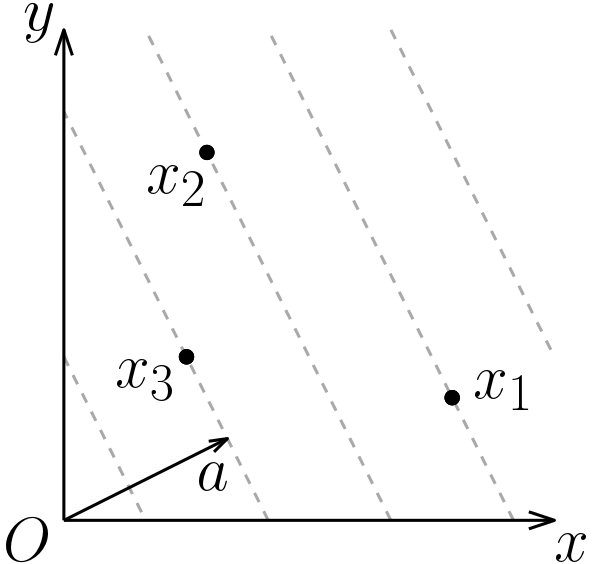
\includegraphics[width=0.2\textwidth]{figures/def2DPref}
    \end{center}
    \ \caption{
      The ``level sets'' of the preference $>_a$,
      which ranks outcomes according to distance from the origin along
      direction $a$.
    }
  \end{wrapfigure}
  Let $\{x_1,\ldots,x_m\} = X\subseteq \Rgz^d$ be any set of
  $m$ distinct points with nonnegative coordinates.
  We call $X$ the set of \emph{outcomes}.
  Given any $a\in \Rgz^d$, which we call a \emph{preference weight},
  define a order $>_a$ on $X$ as follows:
  $x_i >_a x_j$ if and only if $\ip{a}{x_i} > \ip{a}{x_j}$.
  Let $R(X)$ denote the set of total orders on $X$.
  Define
  \begin{align*}
    P_d(X) = \{ \succ \in R(X) | \exists a\in\Rgz^d: x \succ y \iff x >_a y\}
  \end{align*}
  Note that we consider only total orders, in particular,
  ties are not allowed.
  % This maybe could use a footnote:
  % \footnote{
  %   This is largely without loss of generality.
  %   For a given $x,y$ pair, the set of $a$ for which
  %   $\ip{a}{x} = \ip{a}{y}$ has measure zero.
  % }

  Some first observations:
  \begin{itemize}
    \item If $d=1$, then $|P(X)| = 1$, i.e. preferences are completely
      determined by the underlying set $X$.
    \item If $d=n$, then every linear preference on $X$ can occur in $P(X)$.
      \begin{proof}
        Let $X = \{e_i\}$ simply be the standard basis vectors.
        To induce an ordering $i_1, i_2, \ldots, i_n$, just create a preference
        vector $a$ which gives weight $1/k$ to coordinate $i_k$.
      \end{proof}
  \end{itemize}
  The above hints that there should be some sort of continuum between $d=1$
  and $d=n$ of how complex a preference set $P_d(X)$ can be.
  We will find that $d=2$ is a particular sweet spot between expressibility and
  simplicity.
  A core piece of intuition to keep in mind for this paper is that
  a collection of $d$-dimensional preferences is really a $d-1$ dimensional space:
  preferences $>_a$ are invariant under $\|a\|$, so without loss of generality
  we can take all preferences to lie on the unit sphere.
  In particular, $2$-dimensional preferences are a well-behaved one dimensional
  space.

\section{Lemmas}
  In this section, we set up the tools needed to reason about 
  $d$-dimensional preferences.

  \subsection{Lemmas based on the structure of $X$}
    These first few lemmas relate geometric properties of $X$ to
    limitations on the structure of $>_a$ for a specific, fixed $a$.

    The most simple way $X$ gives structure to preferences is if
    one outcome is better in all attributes.
    \begin{definition}
      Let $x,y\in X\subseteq \Rgz^d$.
      We say $x$ \emph{dominates} $y$, denoted $x\gg y$,
      if $x[k] > y[k]$ for each $k=1,\ldots,d$.
    \end{definition}
    \begin{proposition}
      If $x \gg y$, then $x >_a y$ for any nonzero $a\in \Rgz^d$.
    \end{proposition}
    \begin{proof}
      Simply observe $a_i x_i \ge a_i y_i$ for each $i=1,\ldots, d$.
      Because $a\ne 0$, there is also some $i$ where $a_i x_i > a_i y_i$.
    \end{proof}

    When comparing different outcomes, a useful tool is
    the familiar geometric notion of a convex hull.
    Intuitively, if a preference weight does not like any of a set of options,
    it will not like any outcome in the hull of those options either.
    Thus, a point ``dominated by the hull'' of a set of options
    (as in figure~\ref{fig:domHull}) cannot be preferred to all those options.
    \begin{definition}
      For points $x_1,\ldots,x_n \in \R^d$, let $\hull(x_1,\ldots,x_n)
      = \{u_1x_1 + \ldots + u_nx_n | 0\le u_i\le 1, \sum_{i=1}^n u_i = 1\}$
      denote the convex hull of $x_1,\ldots,x_n$.
    \end{definition}
    \begin{lemma}\label{lem:agreementHull}
      Let $z,x_1,\ldots,x_k \in \Rgz^d$ and $a\in \Rgz^d \setminus \{0\}$.
      If $z >_a x_i$ for $i=1,\ldots,k$, then $z >_a w$
      for any $w\in \hull(x_1,\ldots,x_k)$.
    \end{lemma}
    \begin{proof}
      We have $\ip{a}{z} > \ip{a}{x_i}$ for each $i=1,\ldots,k$.
      If $w = u_1x_1+ \ldots + u_nx_n$ and $\sum_i u_i =1$, then
      $\ip{a}{w} = u_1\ip{a}{x_1}+\ldots+u_n\ip{a}{x_n}
      < u_1\ip{a}{z} + \ldots + u_n\ip{a}{z} = \ip{a}{z}$.
    \end{proof}

    \begin{proposition}\label{prop:domHull}
      Let $z,x_1,\ldots,x_k \in \Rgz^d$.
      Suppose that there exists $w\in \hull(x_1,\ldots,x_k)$
      such that $w \gg z$.
      Then no $a$ satisfies $z >_a x_i$ for each $i=1,\ldots, k$.
      % Suppose that there exists $w\in \hull(x_1,\ldots,x_k)$
      %     such that $z \gg w$.
      %     Then no $a$ satisfies $x_i >_a z$ for each $i=1,\ldots, k$.
    \end{proposition}
    \begin{proof}
      For contradiction, suppose such an $a$ exists.
      Then $z >_a w$ as well. However, because $w \gg z$,
      this is a contradiction.
    \end{proof}
    Note that lemma~\ref{lem:agreementHull} and proposition~\ref{prop:domHull}
    both hold when you reverse all the inequalities in their statements,
    via the same arguments.

    \begin{figure}[t]
      \centering
      \begin{subfigure}[t]{0.3\textwidth}
        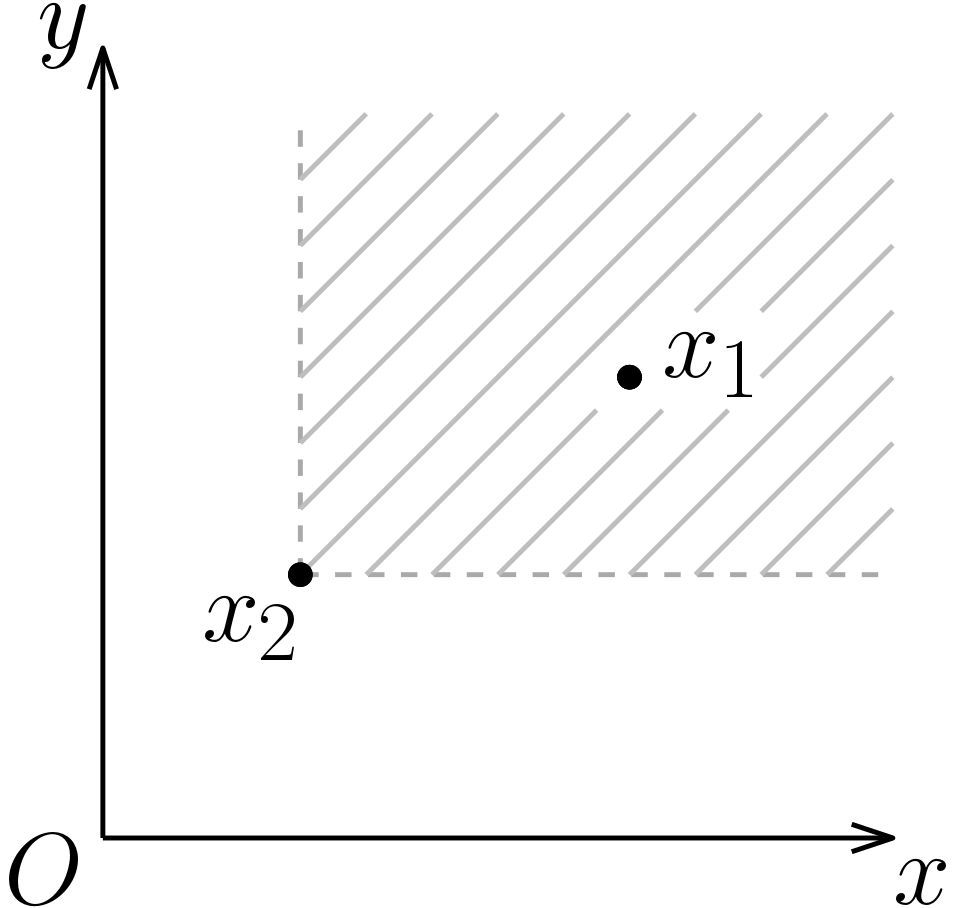
\includegraphics[width=0.9\textwidth]{figures/defDom}
        \caption{$x_1$ dominates $x_2$ ($x_1 \gg x_2$)}
        \label{fig:gull}
      \end{subfigure}
      ~
      \begin{subfigure}[t]{0.3\textwidth}
        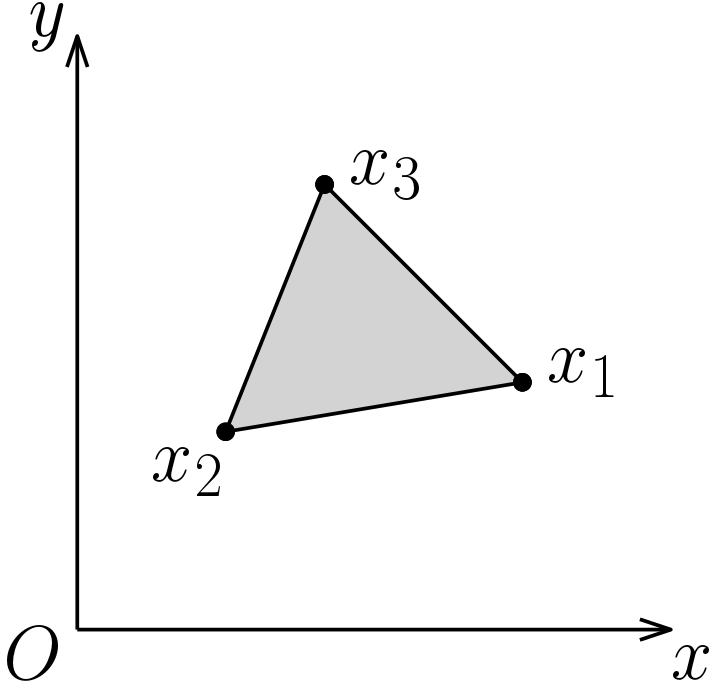
\includegraphics[width=0.9\textwidth]{figures/defHull}
        \caption{The convex $\hull$}
        \label{fig:tiger}
      \end{subfigure}
      ~
      \begin{subfigure}[t]{0.3\textwidth}
        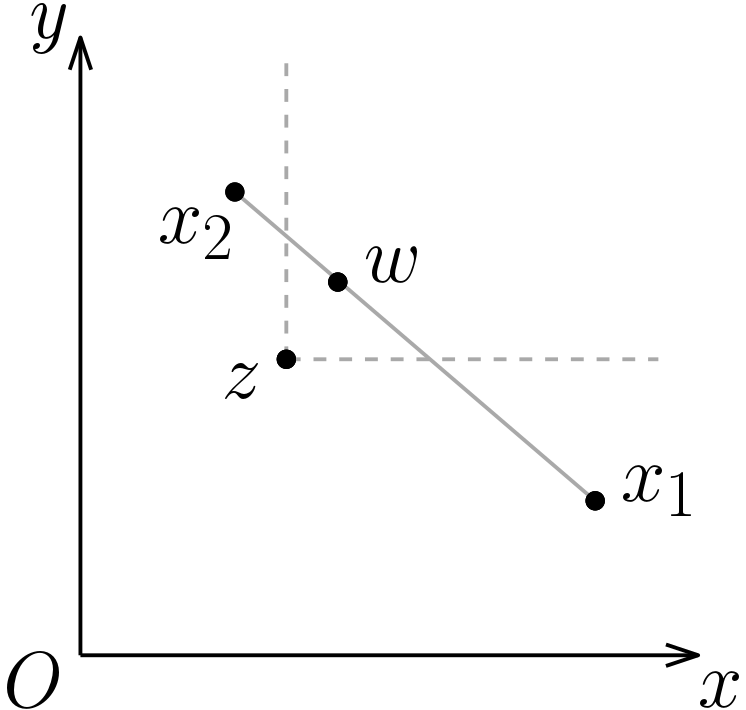
\includegraphics[width=0.9\textwidth]{figures/propDomHull}
        \caption{Proposition~\ref{prop:domHull}}
        \label{fig:domHull}
      \end{subfigure}

      \caption{}\label{fig:animals}
    \end{figure}

  \subsection{Lemma relating different preference vectors}
    \begin{wrapfigure}{r}{0.25\textwidth}
      \vspace{-1.1in}
      \begin{center}
        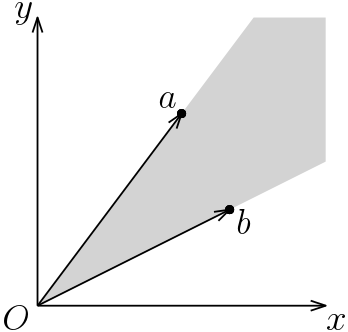
\includegraphics[width=0.28\textwidth]{figures/defCone}
      \end{center}
      \caption{The convex cone}
      \vspace{-1in}
    \end{wrapfigure}

    % This next group of lemmas relates different different preference vectors.
    % They will be very useful for our results about voting schemes.

    When comparing different preference weights, a useful tool is
    the familiar geometric notion of a convex cone.
    Intuitively, if a set of weights agree about a certain preference,
    so does every weight in their cone.
    \begin{definition}
      For any vectors $a_1,\ldots, a_k \in \Rgz^d$, define
      \[ \cone(a_1,\ldots,a_k) = \{ u_1a_1 + \ldots + u_ka_k | u_i\ge 0 \forall j\} \]
    \end{definition}
    \begin{proposition}\label{prop:conesAgreement}
      Suppose that for preference weights $a_1,\ldots, a_k$,
      we have $x >_{a_1} y, \ldots, x >_{a_k} y$.
      Then for any nonzero $b\in \cone(a_1,\ldots, a_k)$,
      $x >_b y$ as well.
    \end{proposition}
    \begin{proof}
      Let $b = u_1a_1+ \ldots + u_ka_k$.
      We get $\ip{b}{x} = u_1\ip{a_1}{x} + \ldots + u_k\ip{a_k}{x}
      > u_1\ip{a_1}{y} + \ldots + u_k\ip{a_k}{y} = \ip{b}{y}$,
      as desired.
    \end{proof}

  \subsection{Lemmas for $2$ dimensional preferences}

    This section turns to our main focus: $2$ dimensional preferences.
    Given two points $x,y$ in our set of outcomes $X$, we give a simple
    classification of which preference weight prefer $x$ and which prefer $y$.
    To do so, we introduce the notion of a weight ``indifferent between $x$ and $y$''.
    \begin{lemma}
      Let $x,y\in \Rgz^2$ be distinct points where neither 
      $x$ nor $y$ dominates the other.
      There exists a unique unit vector $b\in\Rgz^2$ such that
      $\ip{b}{x} = \ip{b}{y}$.
    \end{lemma}
    \begin{proof}
      Without loss of generality let $x_1 < y_1$, $x_2 > y_2$
      (if either of these are equalities, the standard basis vectors
      $e_1$ or $e_2$ will do).
      There exists exactly one unit vector $b$ in $\Rgz^2$ such that
      $b_1 / b_2 = (x_2 - y_2) / (y_1 - x_1)$.
      It's easy to check that this is a necessary and sufficient 
      condition for having $\ip{b}{x} = \ip{b}{y}$.
    \end{proof}
    \begin{definition}
      For $x,y\in \Rgz^2$ where neither dominates the other,
      let the ``indifferent vector of $x$ and $y$'',
      denoted $\indif(x,y)$, be the unit vector $b\in\Rgz^2$ such 
      that $\ip{b}{x} = \ip{b}{y}$.
    \end{definition}

    \begin{wrapfigure}{r}{0.3\textwidth}
      \vspace{-0.4in}
      \begin{center}
        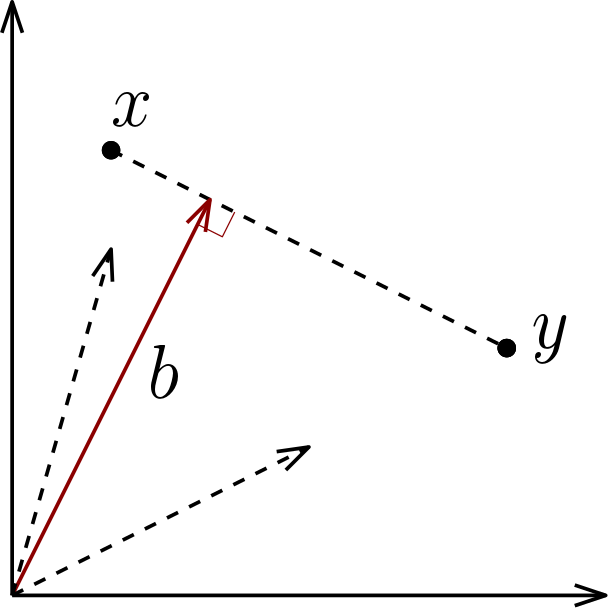
\includegraphics[width=0.26\textwidth]{figures/clmAngle}
      \end{center}
      \caption{
        Proposition~\ref{prop:compEqualizerAngle}. $b=\indif(x,y)$.
        Preferences above $b$ (those with higher angle) all prefer $x$,
        and those below $b$ (those with lower angle) all prefer $y$
      }
      \vspace{-0.7in}
    \end{wrapfigure}

    This next lemma says that the indifference vector of $x$ and $y$ divides 
    the space of preferences into two halves: one that prefers $x$, one that
    prefers $y$. This division is given by another very natural ordering,
    this one for preference weights. The following definition has an obvious
    interpretation by considering $\theta(a)$ to be the angle of $a$ from the
    positive $x$ axis, but we use an equivalent algebraic definition to simply
    our proofs.
    Of course, feel free to ignore this definition, and just use the more
    natural interpretation of $\theta(\cdot)$ as a function which gives the angle.

    \begin{definition}
      We say $a$ has a larger angle than $b$, denoted $\theta(a) > \theta(b)$,
      if $a_2 / a_1 > b_2 / b_1$.
      % If one of those quotients is not defined,
      % $\theta(a) > \theta(b)$ if $a_1 = 0$ and $b_1 \ne 0$.
      % (  $a \times b = a_1 b_2 - a_2 b_1 < 0$.  )
    \end{definition}
    % To see that this definition is equivalent to the natural analogue about the
    % angle from the positive $x$ axis, just consider the ``slopes'' of the
    % vectors $a$ and $b$. Our definition of $\theta(a) > \theta(b)$
    % means $a_2 / a_1 > b_2 / b_1$ (in all but some edge cases).

    \begin{proposition} \label{prop:compEqualizerAngle}
      Consider any pair of points $x, y \in \Rgz^2$, 
      where $x_1 < y_1$ and $x_2 > y_2$, 
      and let $b = \indif(x,y)$.
      Then for any preference weight vector $a \in \R_{\geq 0}^2$,
      \begin{enumerate}
        \item \label{clm:angle1} $\theta(a) > \theta(b)$ if and only if $x >_a y$.
        \item \label{clm:angle2} $\theta(a) < \theta(b)$ if and only if $y >_a x$.
      \end{enumerate}
    \end{proposition}
    \begin{proof}
      Except for the edge case where one vector is a
      multiple of the other, the two items are exactly the same statement.
      We prove the first one:
      \begin{align*}
        x >_a y
        & \iff a_1 x_1 + a_2 x_2 > a_1 y_1 + a_2 y_2
        \\ & \iff \frac{a_2}{a_1} > \frac{y_1 - x_1}{x_2 - y_2} 
          = \frac{b_2}{b_1}
        \\ & \iff 0 > a_1 b_2 - a_2 b_1
        \\ & \iff \theta(a) > \theta(b)
      \end{align*}
    \end{proof}

    % For completeness, we prove the following simple result:
    % \begin{proposition}
    %   If $\theta(a) < \theta(u) < \theta(b)$, then $u\in \cone(a,b)$.
    % \end{proposition}

\clearpage % NOTE: maybe not
\section{Bounding the number of $2$-dimensional preferences}

  \begin{wrapfigure}{r}{0.3\textwidth}
    \begin{center}
      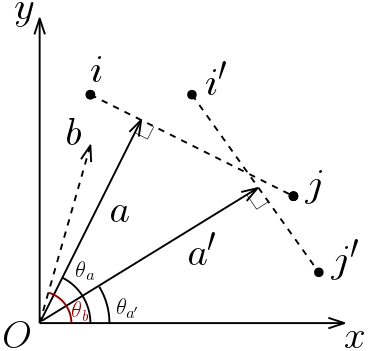
\includegraphics[width=0.28\textwidth]{figures/lemSlopes}
    \end{center}
    \caption{
      Theorem~\ref{thrm:maxNumberTwoD}.
      Indifference vectors $b$ and $b'$ divide preference weight into three
      regions, which each have the same preferences for $x$ vs. $y$
      and $x'$ vs. $y'$.
    }
  \end{wrapfigure}

  We are able to obtain a tight upper bound on the number of distinct linear
  preferences which arise from a given two-dimensional outcome set $X$.
  In particular, note that $|P_2(X)|$ is much less than $m!$, the total number
  of linear orders on $X$.
  \begin{theorem} \label{thrm:maxNumberTwoD}
    Let $X\subseteq \Rgz^2$ with $|X| = m$. We have
    \[ \sizeof{P_2(X)} \leq \binom{m}{2} + 1 \]
  \end{theorem}
  \begin{proof}
    Consider the following set of preference weights:
    \[ B = \{ \indif(x,y) | x,y\in X\text{ and neither dominates the other} \} \]

    Consider the different regions of $\Rgz^2$ separated by elements of $B$.
    That is, consider the equivalence classes of the relation $\sim$
    on $\Rgz^2\setminus B$, where $a \sim a'$
    means that $\forall b\in B: \theta(a) < \theta(b) \iff \theta(a') < \theta(b)$.
    We claim that if $a\sim a'$, then $x >_a y \iff x >_{a'} y$ for all $x,y\in X$.
    Proof: If $x \gg y$ or $y \gg x$, the order between $x$ and $y$ fixed for
    any $a$. Otherwise, $\indif(x,y)\in B$, so
    by proposition~\ref{prop:compEqualizerAngle}, this means
    $x >_a y \iff x >_{a'} y$.

    Thus, the mapping from $\Rgz^2 \to R(X)$ given by $a\mapsto (>_a)$ is constant
    on equivalence classes of $\sim$. This map is surjective by definition.
    Furthermore, $a,a'$ in distinct equivalence classes of $\sim$
    give distinct preferences $>_a, >_{a'}\in R(X)$, again by
    proposition~\ref{prop:compEqualizerAngle}, because $a$ and $a'$ are on a
    different side of some $b\in B$ under the $\theta$ order.
    Thus, there is a bijection between equivalence classes of $\sim$ and
    preferences in $P_2(X)$.

    Note that $|D|\le {m \choose 2}$, so $\sim$ divides the $\Rgz^2$ into at most
    ${m \choose 2}+1$ regions based on the $\theta$ order.
    Thus $\sizeof{P_2(X)} \leq \binom{m}{2} + 1$, as desired.
  \end{proof}

  Furthermore, this upper bound is tight.
  Notice that the proof of the upper bound gives a simple condition for the
  upper bound to be tight: no point of $X$ should dominate another,
  and every pair of points $x,y\in X$ should give a distinct indifference
  vector $\indif(x,y)$.
  To construct such an $X$ with $m$ outcomes, consider
  $X' = \{ (i,m + 1 - i) | i=1,\ldots,m \}$, and randomly perturb each point a
  bit such that all $\indif(x,y)$ vectors are distinct\footnote{
    If you want to get really abstract and fancy, let
    $\alpha_1,\ldots, \alpha_n$ be real numbers which are
    algebraically independent over $\mathbb Q$, and such that
    $|\alpha_i| < 1/3$. Then the points $\{(i,m + 1 - i + \alpha_i)\}_{i=1}^m$
    cannot possibly yield a repeated indifference vector, by
    algebraic considerations.
  }.

\section{Impossibility Results}

  \subsection{Large preference cycles are impossible in any dimension}
    The following preference set may be important in high dimension.
    We call it $k$-{\sc Cycle}:
    % \begin{align*}
    %   1 > 2 > 3 > 4 \\
    %   2 > 3 > 4 > 1 \\
    %   3 > 4 > 1 > 2 \\
    %   4 > 1 > 2 > 3 \\
    % \end{align*}
    \begin{align*}
      \begin{array}{ccccccccccccccccccccccccccccccccccccccccc}
      1 &>& 2 &>& 3 &>&\ldots &>& k-2 &>& k-1 &>& k \\
      2 &>& 3 &>& 4 &>& \ldots &>& k-1 &>& k &>& 1 \\
      3 &>& 4 &>& 5 &>& \ldots &>& k &>& 1 &>& 2 \\
        &&    &&    &&   \vdots \\
      k-1&>&k&>& 1 &>&\ldots &>& k-4 &>& k-3 &>& k-2\\
      k &>& 1 &>& 2 &>& \ldots &>& k-3 &>& k-2 &>& k-1 \\
      \end{array}
    \end{align*}
    \begin{theorem}\label{thrm:noBigCycles}
      $(d+1)$-{\sc Cycle} is not $d$-dimensional for any $d$.
    \end{theorem}
    \begin{proof}
      Suppose for contradiction there existed
      $a_1,\ldots,a_{d+1}\in\Rgz^{d}$ such that $>_{a_i}$ yielded the $i$th line of
      $(d+1)$-{\sc Cycle} (in particular, the line whose favorite point is $i$).
      The vectors $\{a_i\}$ cannot be linearly independent.
      Thus, there exists a linear combination of vectors
      $u_1 a_1 + \ldots + u_{d+1} a_{d+1} = 0$.
      Let $S = \{a_i | u_i > 0\}$ and let $T = \{a_i | u_i < 0\}$.
      Note that, because every coordinate of each $a_i$ is nonnegative
      (and no $a_i$ is zero) neither $S$ nor $T$ are empty.
      We have
      \[ \sum_{a_i \in S} u_i a_i = \sum_{a_i \in T} -u_i a_i \]
      Denote this above vector by $b$, and note that 
      $b\in\Rgz^{d} \setminus \{0\}$ and $b\in \cone(S) \cap \cone(T)$.

      We claim that $b$ satisfies the following:
      \[ 1 >_b 2 >_b 3 >_b \ldots >_b d >_b d+1 >_b 1 \]
      Proof: For each pair $i > i+1$,
      observe that the inequality is satisfied for all the vectors $a_i$ except
      for one of them (namely, $a_{i+1}$ which ranks $i+1$ highest).
      Thus, for either $S$ or $T$, every vector $a_i$ in the set has the opinion
      $i >_{a_i} i+1$. Thus, every vector in the cone of that set
      has the opinion $i > i+1$ as well, by proposition~\ref{prop:conesAgreement}.
      In particular, $i >_b i+1$.
      Of course, the above argument works for the pair $d+>1$ as well.

      Thus, transitivity gives us $1>_b 1$, a contradiction.
    \end{proof}
    This is one of our few results which work for any dimension.
    We'll see that $3$-{Cycle} being impossible for $2$ dimensional preferences
    is a necessary condition for many of the nice properties of $2$ dimensional
    preferences (especially theorem~\ref{thrm:2DCondorcet}).
    Intuitively, it is possible that ``cyclic disagreements'' are a core issue for
    different applications with ordinal preferences (we consider voting here, but
    other cases include matching or resource allocation).
    The impossibility of the $d+1$ cycle in $d$ dimensions gives a
    very nice example of preference sets getting more complicated as
    dimension increases.


  \subsection{Combinatorial impossibilities for $2$ dimensional preferences}

    \begin{proposition}\label{prop:noAllBestWorst}
      Let $P = P_2(X)$ be any set of $2$ dimensional preferences,
      where $|X| \ge 3$.
      It is not possible for every $x\in X$ to be both the
      favorite and least favorite outcome of some preference in $P$.
    \end{proposition}
    \begin{proof}
      If any point dominates another, then the dominated point cannot be favorite.
      Thus we may assume that no point in $X$ is dominated
      by any other point. Pick two points $x \ne y$ such that $x$ has the largest
      first coordinate (i.e. $x_1$) among all of $X$, and $y$ has the highest second
      coordinate (i.e. $y_2$).
      Consider figure~\ref{fig:noAllBestWorst}.
      Any remaining point $z\ne x,y$ must lie in region $1$ or $2$, as all other
      regions either violate the assumption that $x_1 > z_1$ and $y_2 > z_2$
      or cause one point to dominate another.
      If $z$ lies in region $1$, it can never be the favorite, by
      proposition~\ref{prop:domHull}, because it is dominated by some point in
      $\hull(x,y)$.
      If $z$ lies in region $2$, it can never be the least favorite, this time
      by the opposite but completely analogous version of 
      proposition~\ref{prop:domHull}, because $z$ dominates a point in $\hull(x,y)$.
      For the corner case where $z\in\hull(x,y)$, observe that $z$ is
      \emph{always} the middle option among $x$ and $y$.
    \end{proof}

    \begin{wrapfigure}{r}{0.2\textwidth}
      \begin{center}
        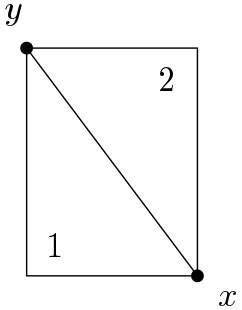
\includegraphics[width=0.2\textwidth]{figures/noBestWorst}
      \end{center}
      \caption{Proposition~\ref{prop:noAllBestWorst}}
      \label{fig:noAllBestWorst}
    \end{wrapfigure}

    This proposition, combined with Theorem~\ref{thrm:noBigCycles}, gives a
    complete combinatorial classification of two dimensional preferences on
    exactly three outcomes. Consider all preferences on three outcomes,
    organized with the two copies of $3$-{\sc Cycle} in different columns.
    \begin{align*}
      1 > 2 > 3 && 1 > 3 > 2 \\
      2 > 3 > 1 && 3 > 2 > 1 \\
      3 > 1 > 2 && 2 > 1 > 3 \\
    \end{align*}
    In order to make our preference set $2$ dimensional, we need to exclude one
    preference from each cycle.
    By relabeling, we can without loss of generality assume that the
    preference with $1 > 2 > 3$ is not in $P$, and consider removing a
    preference from the other cycle.
    If $1 > 3 > 2$ or $2 > 1 > 3$ are removed from $P$, then $P$ will not
    violate proposition~\ref{prop:noAllBestWorst}\footnote{
      We will see later in section~\ref{sec:singleVsTwoD}
      that these preference sets are $2$ dimensional. Up to relabeling, they are
      {\sc BadCompromise} and {\sc GoodCompromise}, respectively.
    }.
    If we only remove $3 > 2 > 1$, then every outcome is some preference's
    favorite and some other preference's least favorite\footnote{
      This gives {\sc Sandwich} from section~\ref{sec:singleVsTwoD}.
    }.
    So this $P$ is not two dimensional.

    % \begin{theorem}
    %   A set of preferences $P$ on exactly three outcomes is $2$ dimensional if
    %   and only if it does not contain $3$-{\sc Cycle} or {\sc Sandwich} 
    %   (up to relabeling).
    % \end{theorem}
    % \begin{proof}
    %   We have seen that $3$-{\sc Cycle} and {\sc Sandwich} are not $2$
    %   dimensional.
    %   Thus, it suffices to show that for any set of preferences which does not
    %   contain a $3$-{\sc Cycle}, the only way for the preference set to
    %   fail to be $2$ dimensional is if it contains {\sc Sandwich}.

    %   The following lists all preference on three outcomes, organized by column
    %   into the two copies of $3$-{\sc Cycle} they form.
    %   \begin{align*}
    %     1 > 2 > 3 && 1 > 3 > 2 \\
    %     2 > 3 > 1 && 3 > 2 > 1 \\
    %     3 > 1 > 2 && 2 > 1 > 3 \\
    %   \end{align*}
    %   At least one element from each of these cycles must not be present in $P$.
    %   By relabeling, we can without loss of generality assume that the
    %   preference with $1 > 2 > 3$ is not in $P$.
    %   Now, we simply need to look at three cases based on which element of the
    %   other cycle is not in $P$.
    %   \begin{itemize}
    %     \item Suppose $1 > 3 > 2$ is not in $P$.
    %       Up to relabeling, all the remaining preferences form a copy of
    %       {\sc BadCompromise}, where $1$ is the point which is never a voter's
    %       favorite.
    %     \item Suppose $3 > 2 > 1$ is not in $P$.
    %       In this case, the remaining preferences form a copy of {\sc Sandwich},
    %       where $3$ is the outcome which is always either favorite or least
    %       favorite.
    %     \item Suppose $2 > 1 > 3$ is not in $P$.
    %       Up to relabeling, all the remaining preferences form a copy of
    %       {\sc GoodCompromise}, where $2$ is the point which is never a voter's
    %       least favorite.
    %   \end{itemize}
    % \end{proof}

  % \subsection{A necessary algorithmic condition for $2$ dimensional preferences}
  %   ((WE BELIEVE THAT THE MATERIAL ABOUT SLOPES MAY PROVIDE A MORE GENERAL
  %   COMBINATORIAL CLASSIFICATION OF 2D PREFS. SHOW SOME NECESSARY CONDITIONS WE
  %   CAN PROVE. CONJECTURE THAT A RELATED THING IS AN IFF))

  %   algorithm:

  %   consider all pairs x,y. If one never exceeds the other, drop it.

  %   For all pairs of tuples, define (x,y) >*> (x',y') if whenever x>y,
  %   we have x'>y'.

  %   I THINK the digraph on such tuples should connected and acyclic if it's two
  %   dimensional.

  %   Optimization:
  %   Pick an arbitrary remaining pair x,y and add the ordered tuple (x,y)
  %   to a set. For all other x',y', add two tuples: (x',y') and (y',x').
  %   If the component containing (x,y) is acyclic, you're good.













\clearpage
%============================================================
%============================================================
\part{Voting With $2$ Dimensional Preferences}

\section{Definitions}
  \subsection{Voting}
    Consider a set of preferences $P$ (i.e. linear orders) on a
    set of outcomes $M$.
    We follow the convention that $m$ is the number of outcomes and $n$
    is the number of voters.
    We have the following definitions:
    \begin{itemize}
      \item A \emph{social welfare function on $P$}
        is a function $F : P^n \to P$
      \item A \emph{social choice function on $P$}
        is a function $f : P^n \to M$. We also call such an $f$ a 
        \emph{voting scheme} or a \emph{voting rule}.
      \item A welfare function $F$ is \emph{unanimous} if,
        for any $\succ\ \in P$, we have $F(\succ,\ldots,\succ) =\ \succ$
      % \item A choice function $f$ is \emph{unanimous} if,
      %   whenever there exists a fixed $a$ with $a \succ_i b$ for all 
      %   $i=1,\ldots, n$ and $b\in M\setminus \{a\}$,
      %   we have $f(\succ_1,\ldots,\succ_n) = a$.
      %   I'm not sure if this is a standard notion.
      \item A welfare function $F$ is a \emph{dictatorship} if
        there exists an $i$ such that $F(\succ_1,\ldots,\succ_n) = \succ_i$
      \item A choice function $f$ is a \emph{dictatorship} if
        there exists an $i$ such that $f(\succ_1,\ldots,\succ_n) = a_i$,
        where $a_i$ is the favorite outcome of $\succ_i$
      \item A welfare function $F$ satisfies \emph{independence of
        irrelevant alternatives} (IIA) if, whenever $a\succ_i b \iff a\succ_i' b$
        and $\succ = F(\succ_1,\ldots,\succ_n),
        \succ' = F(\succ'_1,\ldots,\succ'_n)$,
        we get $a\succ b \iff a\succ' b$. \\
        That is, if no voter changes their opinion between $a$ and $b$,
        the group preference between $a$ and $b$ does not change.
      \item A choice function $f$ is \emph{incentive compatible} if,
        for any $\succ_1,\ldots,\succ_n, i, \succ_i'$, we have \\
        $f(\succ_1,\ldots,\succ_i,\ldots,\succ_n) 
        \succeq_i f(\succ_1,\ldots,\succ_i',\ldots,\succ_n)$ \\
        That is, no voter can get an outcome he strictly prefers by giving a
        false input to $f$.
      \item A collection of preferences $\succ_1,\ldots,\succ_n$,
        has a Condorcet winner $x \in M$ if, for any other $y\in M$,
        we have $x \succ_i y$ for more than half of the indices
        $i=1,\ldots,n$
    \end{itemize}

    Let $R(M)$ denote the set of all linear orders on $M$.
    Recall that when $P = R(M)$, there are many known impossibility results,
    the two most famous of which are:

    \begin{theorem}[Arrow's Impossibility Theorem \cite{AgtBookMechDesignInto}]
      If $|M| \ge 3$, then
      every unanimous social welfare function on $R(M)$
      which satisfies independence of irrelevant alternatives is a dictatorship.
    \end{theorem}

    \begin{theorem}[Gibbard Satterthwaite \cite{AgtBookMechDesignInto}]
      If $|M| \ge 3$, then
      every surjective, incentive compatible social choice function on $R(M)$
      is a dictatorship.
    \end{theorem}

  \subsection{Single-peaked preferences}
    Our main point of contrast will be the well-understood class of
    \emph{single peaked} preferences.

    Let $S\subseteq [0,1]$ be a finite set of $m$ points in the unit interval.
    We call $S$ the set of \emph{outcomes}.
    Let $R(S)$ denote the set of linear orders on $S$.
    A preference $\succ \in R(S)$ is called \emph{single peaked} if
    there exists an outcome $p\in S$ (called the ``peak'' of $\succ$)
    such that $x < y < p \implies x \prec y$ and $p < y < x \implies x \prec y$.
    In other words, the preference has a favorite outcome,
    and its opinion strictly decreases as you move farther away from the favorite.
    Note that no assumption is made about outcomes on different sides of the peak.
    Define

    \begin{align*}
      P_{sp}(S) = \{ \succ \in R(S) | \succ \text{is single peaked }\} && \ 
    \end{align*}
    \begin{wrapfigure}{r}{0.3\textwidth}
      \vspace{-0.75in}
      \begin{center}
        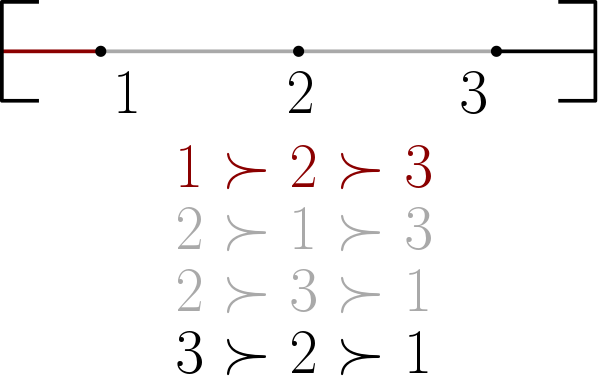
\includegraphics[width=0.3\textwidth]{figures/defSP}
      \end{center}
      \caption{All single peaked preferences on $3$ outcomes}
      \label{fig:singlePeakedThree}
    \end{wrapfigure}

    Single-peaked preferences are studied because the order structure on $S$
    gives a natural voting mechanism: poll voters asking for their favorite
    outcome, i.e. their peak, and output the median peak.
    It is know that this voting scheme satisfies independence of irrelevant
    alternatives (so Arrow's theorem does not hold
    \cite{AgtBookMechDesignInto}) and that this voting scheme is incentive
    compatible (so Gibbard Satterthwaite does not hold \cite{AgtBookNoMoney}).
    As we will see, a voting scheme inspired by this will perform well for
    $2$-dimensional preferences, achieving the same positive results as
    single-peaked preferences.

\section{Single-peaked verses $2$-dimensional preferences}
  \label{sec:singleVsTwoD}

  % TODO: at end, put this at start of whichever page makes the most sense

  When there are exactly three outcomes, $2$-dimensional
  preferences have strictly more expressive power than
  single-peaked preferences.
  \begin{proposition}
    Every single-peaked preference set on $m=3$ outcomes
    is a $2$-dimensional preference set. In particular,
    up to relabeling it is a subset of $P_2(X)$, for
    $X = \{ (3,0), (2,2), (0,3) \}$.
  \end{proposition}
  \begin{proof}
    Without loss of generality, relabel the outcomes
    of the single peaked preferences as $S = \{1,2,3\}$.
    The resulting preferences, as shown in figure~\ref{fig:singlePeakedThree},
    are given by {\sc GoodCompromise}.
  \end{proof}
  Furthermore, {\sc BadCompromise} gives an example of a preference set
  which is $2$-dimensional, but not single-peaked:
  \begin{proposition} \label{prop:noLeastFavorite}
    In a single peaked set of preferences, it is not possible
    for every outcome to be the lowest ranked outcome of some preference.
  \end{proposition}
  \begin{proof}
    The median outcome (via the standard order on $[0,1]$)
    cannot be the lowest ranked.
  \end{proof}

  \begin{figure}[h]
    \centering
    \begin{subfigure}[t]{0.45\textwidth}
      \begin{minipage}{0.55\textwidth}
        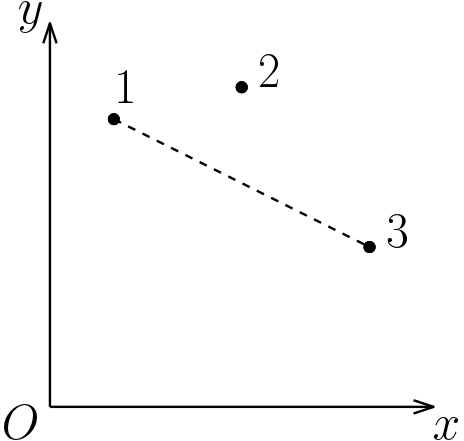
\includegraphics[width=0.9\textwidth]{figures/exGoodComp}
      \end{minipage}\hfill
      \begin{minipage}{0.45\textwidth}
        \begin{align*}
          1 > 2 > 3 \\
          2 > 1 > 3 \\
          2 > 3 > 1 \\
          3 > 2 > 1 \\
        \end{align*}
      \end{minipage}
      \caption{{\sc GoodCompromise}}
      \label{fig:gull}
    \end{subfigure}
    \quad \quad \quad
    \begin{subfigure}[t]{0.45\textwidth}
      \begin{minipage}{0.55\textwidth}
        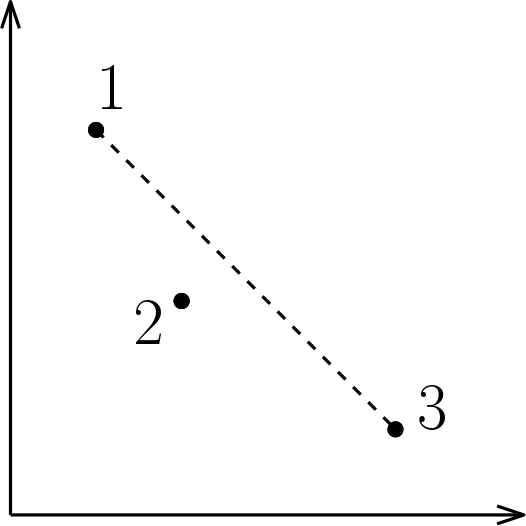
\includegraphics[width=0.9\textwidth]{figures/exBadComp}
      \end{minipage}\hfill
      \begin{minipage}{0.45\textwidth}
        \begin{align*}
          1 > 2 > 3 \\
          1 > 3 > 2 \\
          3 > 1 > 2 \\
          3 > 2 > 1 \\
        \end{align*}
      \end{minipage}
      \caption{\textsc{BadCompromise}}
      \label{fig:gull}
    \end{subfigure}
  \end{figure}

  When $m>3$, neither single-peaked nor $2$-dimensional preferences
  are a subset of the other. One way to see this is to simply
  count the number of single-peaked preferences, and see that it
  grows much faster with $m$ than $2$-dimensional preferences
  (recall that we showed in theorem~\ref{thrm:maxNumberTwoD}
  that the maximal size of a $2$-dimensional
  preference set is $O(m^2)$).
  \begin{proposition}
    The number of single-peaked preferences for any set $S$ of $m$ outcomes
    is at least $2^{\Omega(m)}$
  \end{proposition}
  \begin{proof}
    Choose the median outcome of $S$ to be the peak.
    Given a subset $T\subseteq [m-1]$ of size $|T| = \lfloor m/2\rfloor$,
    we can associate a
    unique single-peaked preference as follows:
    treat the preference as an array of outcomes, ranked highest to lowest.
    Put the median of $S$ at index $0$.
    Let the outcomes to the left of the median occupy the indices corresponding
    to set $T$, and let those to the right occupy the other indices.
    There are ${m-1 \choose \lfloor m/2\rfloor } \ge 2^{\Omega(m)}$ such
    subsets $T$.
  \end{proof}

  \begin{wrapfigure}{r}{0.2\textwidth}
    \centering
    {\textsc{FlipFlop}}
    \begin{align*}
      1 > 2 > 3 > 4 \\
      1 > 2 > 4 > 3 \\
      2 > 1 > 3 > 4 \\
      2 > 1 > 4 > 3 \\
    \end{align*}
    \vspace{-1in}
  \end{wrapfigure}

  A cleaner, more constructive way to see this is the following proposition
  \begin{proposition}
    The preference set {\sc FlipFlop} is single-peaked, but not
    $2$-dimensional.
  \end{proposition}
  \begin{proof}
    To obtain a single-peaked representation, order the outcomes
    from left to right as follows: $3,1,2,4$.
    All preferences will then be possible with peak $1$ or $2$.

    Now we show that {\sc FlipFlop} is not $2$-dimensional.
    Note that neither $1$ nor $2$ can dominate the other,
    and the same holds for $3$ and $4$.
    So let $a=\indif(1,2)$ and $b=\indif(3,4)$.
    % Suppose $\theta(a) < \theta(b)$ (the other case is symmetric).
    Without knowing the outcome space $X\subseteq \Rgz^2$,
    we can't tell which side of $a$ corresponds to $1 > 2$
    verses $2 > 1$ (same with $b$).
    However, we do know that at least one of the following implications should
    hold for any preference $>$ over $X$:
    \begin{align*}
      1 > 2 \implies 3 > 4
      && 1 > 2 \implies 4 > 3 &&
      2 > 1 \implies 3 > 4
      && 2 > 1 \implies 4 > 3
    \end{align*}
    For example, if $\theta(a) < \theta(b)$ and preference weights with smaller
    angle than $a$ (resp. $b$) favor $1 > 2$ (resp. $3 > 4$),
    then $1 > 2 \implies 3 > 4$.

    However, none of these implications are satisfied by the entire preference
    set {\sc FlipFlop}. Thus {\sc FlipFlop} cannot be $2$-dimensional.
  \end{proof}

  When considering restricted domains of preference, it is perhaps more
  important to consider which preference sets \emph{do not} fall into that
  domain. Indeed, if too many preferences are possible, then the impossibility
  results which hold for arbitrary preferences will apply.

  As we've directly shown, $3$-{\sc Cycle} is not $2$ dimensional.
  This is already a good sign: $3$-{\sc Cycle} is a classic example of the
  so-called Condorcet paradox. Despite each preference being a linear order,
  the majority of voters favor $1$ over $2$, $2$ over $3$, and $3$ over $1$.
  That is, ``collective preference'' is cyclic.
  Indeed, $3$-{\sc Cycle} is a preference set with no Condorcet winner,
  and is often used as a basic counterexample for the existence of good voting
  schemes. The fact that cycle is impossible already seems like good news for
  voting schemes on two dimensional preferences.

  Here's another case:
  \begin{proposition}
    {\sc Sandwich} is neither single-peaked nor $2$ dimensional
  \end{proposition}
  \begin{proof}
    {\sc Sandwich} is not single-peaked by proposition~\ref{prop:noLeastFavorite}.
    It's not $2$-dimensional by proposition~\ref{prop:noAllBestWorst}.
  \end{proof}

  \begin{figure}[H]
    \begin{minipage}{0.15\textwidth}
      \centering
      {\textsc{Reverse}}
      \begin{align*}
        1 > 2 > 3 > 4 \\
        4 > 3 > 2 > 1 \\
      \end{align*}
    \end{minipage}\hfill
    \begin{minipage}{0.15\textwidth}
      \centering
      {$3$-\textsc{Cycle}}
      \begin{align*}
        1 > 2 > 3 \\
        2 > 3 > 1 \\
        3 > 1 > 2 \\
      \end{align*}
    \end{minipage}\hfill
    \begin{minipage}{0.15\textwidth}
      \centering
      {\textsc{Sandwich}}
      \begin{align*}
        1 > 2 > 3 \\
        1 > 3 > 2 \\
        3 > 2 > 1 \\
        2 > 3 > 1 \\
      \end{align*}
    \end{minipage}\hfill
    \begin{minipage}{0.55\textwidth}
      \centering
      \begin{tabular}{ r | l }
        $2$-dimensional & {\sc BadCompromise} \\
        single peaked & {\sc FlipFlop}, {\sc NoRep} \\
        both & {\sc Reverse}, {\sc GoodCompromise} \\
        neither & $3$-{\sc Cycle}, {\sc Sandwich} \\
      \end{tabular}
    \end{minipage}\hfill
  \end{figure}

  The above discussion gives a fairly clear picture of the relationship between
  $2$-dimensional and single-peaked preferences.
  While single peaked and $2$-dimensional model noticeably different causes of
  preferences, we argue that $2$-dimensional preferences are in some sense more
  natural. The rest of this section gives some non-formal justification
  for this highly subjective statement.

  In the ``school ranking'' example given in the introduction, the preference of
  students is determined by a single underlying attribute of the student:
  their preference for STEM vs liberal arts.
  In contrast, single-peaked preferences allow voters to have arbitrary
  preferences about outcomes on either side of their peak.
  Two voters with the same peak could have very different preference sets:
  one could like all the points below the peak before any above the peak,
  while the other could simply rank options by distance (for example,
  usual real number distance) from the peak.
  These two voters seem incompatible within the same underlying situation:
  one has a sort of ``hard budget'' at its peak, while the other just
  wants to get close to his favorite.
  A common motivation given for single-peaked preferences is that of political
  policy (with the familiar ``left and right'' manifest literally).
  But why would a voter's favorite policy be the most liberal one which he does
  not hate? This corresponds to the voter who prefers all outcomes right of his
  peak to all those left of his peak.

  Admitedly, for $m \gg 3$, the size of single-peaked preference sets can be
  much larger than that of $2$-dimensional preferences.
  However, we believe that single-peaked preferences still miss certain well
  motivated preference sets, without gaining much essential.
  Indeed, the ordinal preference set {\sc BadCompromise} models the intuitive
  idea of a bad compromise very well: the ``compromise'' outcome $2$ is
  no voter's favorite\footnote{
    Indeed, our voting scheme given in section~\ref{sec:voting} will never
    select outcome $2$ in this case!
  }. However, single-peaked preferences such as {\sc FlipFlop} have no obvious
  interpretation, except for the voters making arbitrary decisions about
  outcomes on different sides of their peak.

\section{Value restriction verses $2$-dimensional preferences}
  \label{sec:VRvsTwoD}

  \begin{figure}[H]
    \begin{minipage}{0.15\textwidth}
      \centering
      {\textsc{MixedCompromise}}
      \begin{align*}
        4 > 3 > 2 > 1 \\
        1 > 2 > 3 > 4 \\
        2 > 1 > 4 > 3 \\
      \end{align*}
    \end{minipage}\hfill
    \begin{minipage}{0.15\textwidth}
      {\textsc{NoRep}}
      \begin{align*}
        3 > 2 > 1 > 4 \\
        1 > 2 > 3 > 4 \\
        2 > 1 > 4 > 3 \\
      \end{align*}
      \centering
    \end{minipage}\hfill
    \begin{minipage}{0.15\textwidth}
      \centering
    \end{minipage}\hfill
  \end{figure}

  With a slightly technical set of points, you can realize
  {\sc MixedCompromise} as a 2D, but neither single peaked nor single caved.
  It isn't single caved, because each of outcome $1,2,3$ is some voter's
  favorite among those three, and it's not single peaked, because among $2,3,4$
  each outcome is some voter's least favorite.

  We denote VR12 as the ``mixed union'' of single peaked and single troughed.

\section{Single-crossing verses $2$-dimensional preferences}
  \label{sec:crossVsTwoD}

  Single-crossing preferences are almost equivalent to $2$-dimensional
  preferences. ((EXPLAIN ORDERING, VOTER REPRESENTATION))

  Here's a key example. The preference set {\sc NoRep} is single peaked, with
  outcomes ordered $3,2,1,4$ from left to right.
  C.f. {\sc MixedCompromise}. Furthermore, the ``majority
  rule'' preference over {\sc NoRep} is $2>1>3>4$, that is, with a single
  voter for each preference of {\sc NoRep}, the majority of voters agree with
  each of the above preferences (and their transitive closure).
  \begin{proposition}
    {\sc NoRep} is not $2$-dimensional
  \end{proposition}
  \begin{proof}
    Suppose for contradiction that the first preference is given by vector $a$,
    the second by $b$, and the third by $c$.
    Consider the $\theta$ ordering relation between $a$, $b$, and $c$.
    Observe the following:
    \begin{itemize}
      \item $a$ cannot be between $b$ and $c$, because $1 >_b 3$, $1 >_c 3$ 
        (and $2 >_b 3$, $2 >_c 3$).
      \item $b$ cannot be between $a$ and $c$, because $2 >_a 1$, $2 >_c 1$.
      \item $c$ cannot be between $a$ and $b$, because $3 >_a 4$, $3 >_b 4$.
    \end{itemize}
  \end{proof}



\section{Voting for $2$-dimensional preferences}
  \label{sec:voting}

  Suppose the set of outcomes $X$ is known.
  Taking inspiration from single-peaked preferences, we define the following
  mechanism for voting:

  \begin{algorithm}
    \caption{Median-angle voting scheme}
    Poll the preference weight $a_i\in\Rgz^d$ from each voter $i$ \\
    Reorder the list $a_i$ by the $\theta$ order, so 
      $\theta(a_i) < \theta(a_{i+1})$ \\
    Return the favorite outcome of the median-angled preference weight
  \end{algorithm}

  \begin{figure}[h]
    \centering
    \begin{subfigure}[t]{0.3\textwidth}
      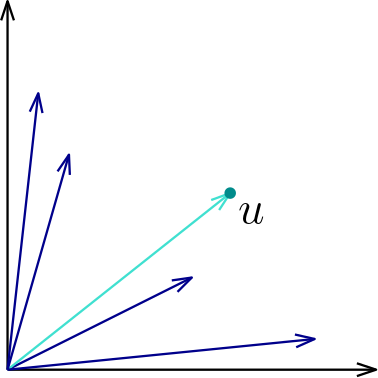
\includegraphics[width=0.9\textwidth]{figures/defMedianAngle}
      \caption{The median-angled preference vector}
      \label{fig:gull}
    \end{subfigure}
    ~
    \begin{subfigure}[t]{0.3\textwidth}
      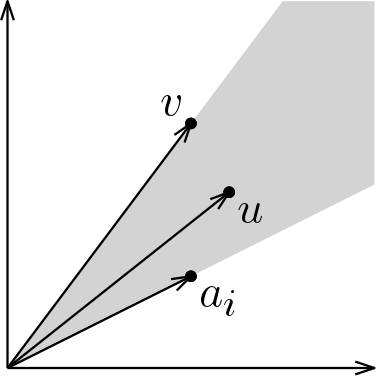
\includegraphics[width=0.9\textwidth]{figures/thrmIncentiveComp}
      \caption{Theorem~\ref{thrm:2DincentiveCompat}}
      \label{fig:tiger}
    \end{subfigure}
    ~
    \begin{subfigure}[t]{0.3\textwidth}
      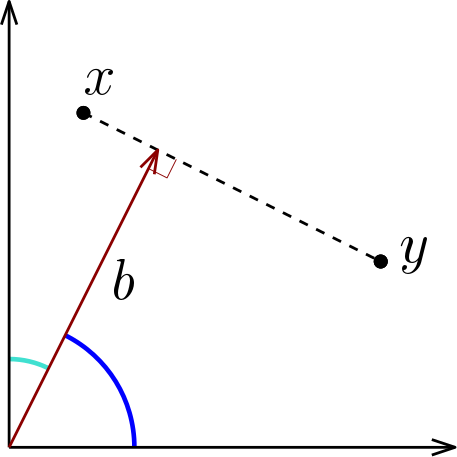
\includegraphics[width=0.9\textwidth]{figures/thrmIIA}
      \caption{Theorems~\ref{thrm:2DIIA} and~\ref{thrm:2DCondorcet}}
      \label{fig:domHull}
    \end{subfigure}

    \caption{}\label{fig:animals}
  \end{figure}

  Intuitively, this seems like a promising voting scheme.
  Preferences are more similar when angles are closer,
  and preference angle gives a continuum between one extreme and the other.
  Thus, the median voter is a natural choice to represent the population.
  It turns out that the framework developed in Part I of this paper gives
  simple proofs of many desirable properties for this voting rule.
  These properties essentially tell us that $2$-dimensional preferences are at
  least as well-behaved as single-peaked preferences.

  Our first result states that a voter cannot strategically manipulate the
  median-angle voting scheme, i.e. the Gibbard Satterthwaite theorem does not
  hold for $2$-dimensional preferences.
  \begin{theorem}\label{thrm:2DincentiveCompat}
    Let the number of voters $n$ be odd.
    The median-angle voting rule for $2$-dimensional preferences
    is incentive compatible.
  \end{theorem}
  \begin{proof}
    Consider any voter $i$ and suppose the voters true preferences 
    are given by weights $a_1,\ldots,a_n$.
    Let $u$ denote the median-angled preference vector chosen when all
    agents report their true preference.
    Suppose $\theta(a_i) < \theta(u)$ (the other case is symmetric).
    The only way in which $i$ can change the median-angled preference vector
    by misreporting his value for $a_i$
    is to \emph{increase} its angle, say to some $\nu$.
    Note that because $\theta(a_i) < \theta(u) < \theta(\nu)$,
    we have $u \in \cone(a_i, \nu)$.
    % Consider any pair $x,y$ such that $x >_{a_i} y$ and $x >_\nu y$,
    % I.e. the manipulated median-angled preference weight agrees with voter $i$.

    For the sake of contradiction, assume $i$ could profit from this
    manipulation, i.e. he could get an outcome he favored chosen by $\nu$.
    Let $y$ be the outcome selected by $u$, and let $x$ be selected by $\nu$.
    We have $x >_\nu y$ and $x >_{a_i} y$.
    By proposition~\ref{prop:conesAgreement}, we get $x >_u y$ as well.
    However, this contradicts the assumption that $u$ selects $y$,
    and completes our proof.
  \end{proof}

  We also define the median-angle social welfare function in the obvious way: if
  the median-angled preference vector is $u$,
  return the linear order $(>_u) \in P_2(X)$
  Given this definition, we see that median-angled voting satisfies independence
  of irrelevant alternatives, and thus Arrow's impossibility theorem does not
  hold for $2$-dimensional preferences.

  \begin{theorem}\label{thrm:2DIIA}
    The median-angle social welfare function satisfies independence of irrelevant
    alternatives.
  \end{theorem}
  \begin{proof}
    Consider any pair of outcomes $x,y$. If either dominates the other, the
    IIA axiom becomes easy to verify.
    So suppose neither dominates the other, without loss of generality take
    $x_1 < y_1$, $x_2 > y_2$, and let $b = \indif(x,y)$.

    Suppose $\{a_i\}$ and $\{a_i'\}$ are collections of preference weights such
    that $x>_{a_i} y \iff x>_{a_i'} y$ for each $i$.
    By proposition \ref{prop:compEqualizerAngle},
    this means that $\theta(a_i) > \theta(b) \iff \theta(a_i') > \theta(b)$.
    Let $u$ denote the median-angled vector among $\{a_i\}$,
    and $u'$ for $\{a_i'\}$.
    Because each pair $a_i, a_i'$ lies on the same side of $b$,
    we must have $u$ and $u'$ on the same side of $b$ as well.
    Thus, $x >_u y \iff x >_{u'} y$, as desired.
  \end{proof}

  The next theorem justifies median-angle voting as \emph{the} natural
  voting scheme for $2$-dimensional preferences, using the notion of a Condorcet
  winner.
  \begin{theorem}\label{thrm:2DCondorcet}
    Among an odd number of $2$-dimensional preferences,
    there is always a Condorcet winner, which is selected
    by the median angle voting scheme
  \end{theorem}
  \begin{proof}
    Let $u$ be the median-angled preference vector, and let
    $x$ be the favorite outcome of $u$.
    Given some outcome $y\ne x$, if $y \ll x$, then
    $y$ is never preferred to $x$.
    So suppose neither $x$ nor $y$ dominate each other, and let
    $b = \indif(x,y)$.
    Let $S$ be the set of preference weights $a$ such that $x>_a y$.
    By proposition~\ref{prop:compEqualizerAngle}, $S$ either consists of all vectors
    $a$ with $\theta(a) > \theta(b)$ or all $a$ with $\theta(a) < \theta(b)$.
    Because $x >_u y$,
    the median angled preference weight $u$ must lie in $S$.
    Thus, more than half of all the input preference weights must lie in $S$.
    Thus, more than half of the input preferences agree that $x > y$.
    Because $y$ was arbitrary, this means $x$ is the Condorcet winner.
  \end{proof}

  We note the following important consequence of the previous theorem:
  if preferences are known to lie in $P_2(X)$ for some $X$,
  but no details about $X$ are known, then a voting protocol can simply
  ask voters for their list of preferences and look for the Condorcet
  winner (note that there is at most one Condorcet winner).
  While it is not immediate that this rule is incentive compatible\footnote{
    This is because it's possible for a manipulative agent to report a
    preference list which is not two dimensional with respect to the set $X$.
    It's possible for such a manipulator to cause there to be no Condorcet
    winner (for example, the preference $1 > 2 > 3$ and $2 > 3 > 1$
    are certainly two dimensional, so the manipulator could report $3 > 1 > 2$
    and create $3$-{\sc Cycle}).
    We conjecture that a single manipulator cannot \emph{change} the Condorcet
    winner, i.e. the manipulated preference set cannot have a Condorcet winner
    different than the original one, but proving this result requires a bit more
    thought.
  } this still gives a good voting rule for honest agents with two dimensional
  preferences.
  % Moreover, it hints that when agents act approximately via a weighted
  % sum of two attributes, it is more likely that there is a Condorcet winner.
  % ((NOTE: CONTEMPLATE THE FOLLOWING HOLE IN THE ABOVE LOGIC:
  % WHAT IF AN AGENT STRATEGICALLY REPORTS A PREFERENCE THAT IS NOT TWO
  % DIMENSIONAL FOR THE UNDERLYING SET X. FOR ONE, THE AGENT MY FORCE THE
  % PROCEDURE TO FAIL BECAUSE IT WON'T HAVE A CONDORCET WINNER. BUT AD HOC 
  % WE DON'T KNOW HE CAN'T MANIPULATE THE CONDORCET WINNER))

  \bibliography{weightedPref}{}
  \bibliographystyle{alpha}
\end{document}
